% =============================================================
% Anhang zu Tag 19 — Werkstatt-Material:
%   1. Log- und Antilog-Tafel für GF(256)
%   2. Farbig markiertes 10×10-Raster für „MUT"
%   3. Farbig markiertes 14×14-Raster für „GESCHAFFT"
%
% Greta nutzt das, weil Drucker fehlen: Tabellen direkt zum
% Nachschlagen im Buch, Raster als Vorbild zum Abmalen auf
% Karopapier.
% =============================================================

\chapter*{Anhang zu Tag 19 — Werkstatt-Material}
\addcontentsline{toc}{chapter}{Anhang zu Tag 19 — Werkstatt-Material}

\begin{quote}
Drucker zur Hand? Dann liegen die einzelnen Werkstattbögen separat im
Release-Asset (siehe Kapitel-Footnotes). \emph{Kein} Drucker? Dann
arbeitest du direkt mit diesem Anhang: die Tabellen schlägst du im
Buch nach, die zwei Raster malst du auf Karopapier ab — die UTAH-L-Form
in Buntstift, dann die schwarzen Bits hinein.
\end{quote}

% --- Log/antilog-Tafel ---------------------------------------------
\section*{Log- und Antilog-Tafel für GF(256)}

Beide Tafeln gehören zum Standard-Setup für Datamatrix ECC-200:
primitives Polynom $0x12D$, Generator-Element $\alpha = 2$.

\paragraph{Multiplikations-Spickzettel}
\[
  a \times b \;=\; \text{antilog}\!\big[(\log[a] + \log[b]) \bmod 255\big]
\]
\textbf{Sonderfälle:} $a \times 0 = 0$, $a \times 1 = a$ (weil $\log[1]=0$).

\paragraph{Lese-Anleitung}
Zeilen-Beschriftung = $16 \cdot r$, Spalten-Beschriftung = $c$.
Der Eintrag im Schnittpunkt ist der Wert $\log[16r + c]$ bzw.\
$\text{antilog}[16r + c]$. Beispiel für die log-Tafel: $\log[73]$
findest du in Zeile~$64$ ($73 = 64 + 9$), Spalte~$9$.

\subsection*{log-Tafel: $\log[v]$ für $v = 1 \dots 255$}

\begin{center}
\footnotesize
\setlength{\tabcolsep}{3pt}
\renewcommand{\arraystretch}{1.05}
\begin{tabular}{r|rrrrrrrrrrrrrrrr}
\toprule
$v$ & \textbf{0} & \textbf{1} & \textbf{2} & \textbf{3} & \textbf{4} & \textbf{5} & \textbf{6} & \textbf{7} & \textbf{8} & \textbf{9} & \textbf{10} & \textbf{11} & \textbf{12} & \textbf{13} & \textbf{14} & \textbf{15} \\
\midrule
\textbf{  0} & --- & 0 & 1 & 240 & 2 & 225 & 241 & 53 & 3 & 38 & 226 & 133 & 242 & 43 & 54 & 210 \\
\textbf{ 16} & 4 & 195 & 39 & 114 & 227 & 106 & 134 & 28 & 243 & 140 & 44 & 23 & 55 & 118 & 211 & 234 \\
\textbf{ 32} & 5 & 219 & 196 & 96 & 40 & 222 & 115 & 103 & 228 & 78 & 107 & 125 & 135 & 8 & 29 & 162 \\
\textbf{ 48} & 244 & 186 & 141 & 180 & 45 & 99 & 24 & 49 & 56 & 13 & 119 & 153 & 212 & 199 & 235 & 91 \\
\textbf{ 64} & 6 & 76 & 220 & 217 & 197 & 11 & 97 & 184 & 41 & 36 & 223 & 253 & 116 & 138 & 104 & 193 \\
\textbf{ 80} & 229 & 86 & 79 & 171 & 108 & 165 & 126 & 145 & 136 & 34 & 9 & 74 & 30 & 32 & 163 & 84 \\
\textbf{ 96} & 245 & 173 & 187 & 204 & 142 & 81 & 181 & 190 & 46 & 88 & 100 & 159 & 25 & 231 & 50 & 207 \\
\textbf{112} & 57 & 147 & 14 & 67 & 120 & 128 & 154 & 248 & 213 & 167 & 200 & 63 & 236 & 110 & 92 & 176 \\
\textbf{128} & 7 & 161 & 77 & 124 & 221 & 102 & 218 & 95 & 198 & 90 & 12 & 152 & 98 & 48 & 185 & 179 \\
\textbf{144} & 42 & 209 & 37 & 132 & 224 & 52 & 254 & 239 & 117 & 233 & 139 & 22 & 105 & 27 & 194 & 113 \\
\textbf{160} & 230 & 206 & 87 & 158 & 80 & 189 & 172 & 203 & 109 & 175 & 166 & 62 & 127 & 247 & 146 & 66 \\
\textbf{176} & 137 & 192 & 35 & 252 & 10 & 183 & 75 & 216 & 31 & 83 & 33 & 73 & 164 & 144 & 85 & 170 \\
\textbf{192} & 246 & 65 & 174 & 61 & 188 & 202 & 205 & 157 & 143 & 169 & 82 & 72 & 182 & 215 & 191 & 251 \\
\textbf{208} & 47 & 178 & 89 & 151 & 101 & 94 & 160 & 123 & 26 & 112 & 232 & 21 & 51 & 238 & 208 & 131 \\
\textbf{224} & 58 & 69 & 148 & 18 & 15 & 16 & 68 & 17 & 121 & 149 & 129 & 19 & 155 & 59 & 249 & 70 \\
\textbf{240} & 214 & 250 & 168 & 71 & 201 & 156 & 64 & 60 & 237 & 130 & 111 & 20 & 93 & 122 & 177 & 150 \\
\bottomrule
\end{tabular}
\end{center}


\subsection*{antilog-Tafel: $\text{antilog}[i] = \alpha^i$ für $i = 0 \dots 254$}

\begin{center}
\footnotesize
\setlength{\tabcolsep}{3pt}
\renewcommand{\arraystretch}{1.05}
\begin{tabular}{r|rrrrrrrrrrrrrrrr}
\toprule
$i$ & \textbf{0} & \textbf{1} & \textbf{2} & \textbf{3} & \textbf{4} & \textbf{5} & \textbf{6} & \textbf{7} & \textbf{8} & \textbf{9} & \textbf{10} & \textbf{11} & \textbf{12} & \textbf{13} & \textbf{14} & \textbf{15} \\
\midrule
\textbf{  0} & 1 & 2 & 4 & 8 & 16 & 32 & 64 & 128 & 45 & 90 & 180 & 69 & 138 & 57 & 114 & 228 \\
\textbf{ 16} & 229 & 231 & 227 & 235 & 251 & 219 & 155 & 27 & 54 & 108 & 216 & 157 & 23 & 46 & 92 & 184 \\
\textbf{ 32} & 93 & 186 & 89 & 178 & 73 & 146 & 9 & 18 & 36 & 72 & 144 & 13 & 26 & 52 & 104 & 208 \\
\textbf{ 48} & 141 & 55 & 110 & 220 & 149 & 7 & 14 & 28 & 56 & 112 & 224 & 237 & 247 & 195 & 171 & 123 \\
\textbf{ 64} & 246 & 193 & 175 & 115 & 230 & 225 & 239 & 243 & 203 & 187 & 91 & 182 & 65 & 130 & 41 & 82 \\
\textbf{ 80} & 164 & 101 & 202 & 185 & 95 & 190 & 81 & 162 & 105 & 210 & 137 & 63 & 126 & 252 & 213 & 135 \\
\textbf{ 96} & 35 & 70 & 140 & 53 & 106 & 212 & 133 & 39 & 78 & 156 & 21 & 42 & 84 & 168 & 125 & 250 \\
\textbf{112} & 217 & 159 & 19 & 38 & 76 & 152 & 29 & 58 & 116 & 232 & 253 & 215 & 131 & 43 & 86 & 172 \\
\textbf{128} & 117 & 234 & 249 & 223 & 147 & 11 & 22 & 44 & 88 & 176 & 77 & 154 & 25 & 50 & 100 & 200 \\
\textbf{144} & 189 & 87 & 174 & 113 & 226 & 233 & 255 & 211 & 139 & 59 & 118 & 236 & 245 & 199 & 163 & 107 \\
\textbf{160} & 214 & 129 & 47 & 94 & 188 & 85 & 170 & 121 & 242 & 201 & 191 & 83 & 166 & 97 & 194 & 169 \\
\textbf{176} & 127 & 254 & 209 & 143 & 51 & 102 & 204 & 181 & 71 & 142 & 49 & 98 & 196 & 165 & 103 & 206 \\
\textbf{192} & 177 & 79 & 158 & 17 & 34 & 68 & 136 & 61 & 122 & 244 & 197 & 167 & 99 & 198 & 161 & 111 \\
\textbf{208} & 222 & 145 & 15 & 30 & 60 & 120 & 240 & 205 & 183 & 67 & 134 & 33 & 66 & 132 & 37 & 74 \\
\textbf{224} & 148 & 5 & 10 & 20 & 40 & 80 & 160 & 109 & 218 & 153 & 31 & 62 & 124 & 248 & 221 & 151 \\
\textbf{240} & 3 & 6 & 12 & 24 & 48 & 96 & 192 & 173 & 119 & 238 & 241 & 207 & 179 & 75 & 150 & --- \\
\bottomrule
\end{tabular}
\end{center}


\bigskip
\paragraph{Beispiel.}
$73 \times 31$:
$\log[73] = 198$, $\log[31] = 234$, Summe $= 432$, mod $255$ $= 177$,
$\text{antilog}[177] = 254$. Also $73 \times 31 = 254$ in GF(256).

\clearpage

% --- Farbig markierte Raster ---------------------------------------
\section*{Datamatrix-Raster mit UTAH-Markierung}

Jedes 8-Bit-Codeword wird als L-förmige UTAH-Form ins Symbol gesetzt
(ISO/IEC~16022, Annex~F). In den folgenden Rastern hat \emph{jedes
Codeword seine eigene Pastell-Farbe}; jedes Modul ist mit
„CW-Nr.\,/\,Bit-Nr." beschriftet.

\paragraph{Empfehlung} Male das Raster auf Karopapier nach
(1~Modul = 1~Karo). Färbe die UTAHs mit Buntstiften — dabei lernst du
den Cursor-Pfad spielerisch. Die schwarzen Datenbits trägst du
\emph{danach} per Bleistift-Schraffur ein, anhand deiner berechneten
Codewords.

\subsection*{10×10-Raster für „MUT" — 8 Codewords}

Innenfläche: 8×8 Module = 64 Bits = 8~Codewords~à~8~Bits (3~Daten +
5~ECC, kein Padding).

\begin{center}
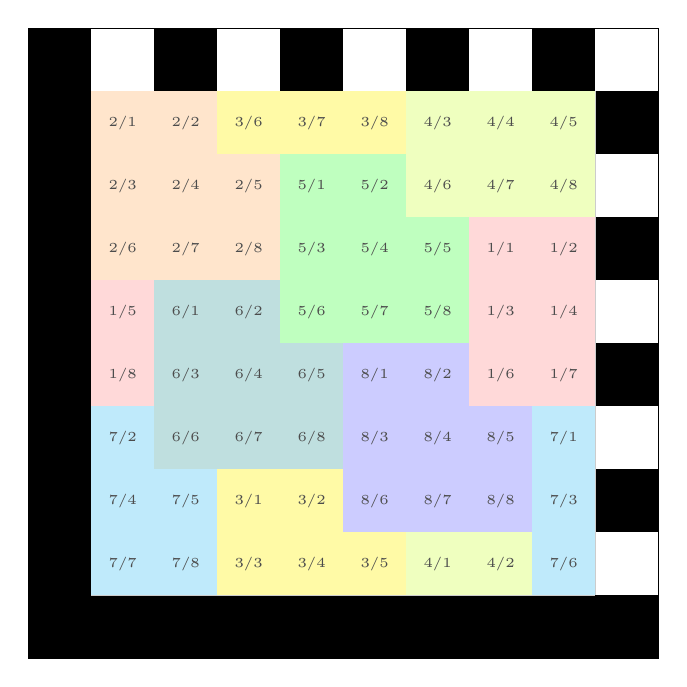
\begin{tikzpicture}[x=8mm, y=-8mm, every node/.style={font=\tiny}]
  % Symbol-Aussenrahmen 10×10
  \draw[black] (0, 0) rectangle (10, 10);
  % L-Pattern: untere Kante (Zeile 9) + linke Kante (Spalte 0)
  \foreach \c in {0,...,9}{ \fill[black] (\c, 9) rectangle (\c+1, 10); }
  \foreach \r in {0,...,8}{ \fill[black] (0, \r) rectangle (1, \r+1); }
  % Zeitsignal: obere Kante (gerade Spalten), rechte Kante (ungerade Zeilen)
  \foreach \c in {0, 2, 4, 6, 8}{ \fill[black] (\c, 0) rectangle (\c+1, 1); }
  \foreach \r in {1, 3, 5, 7}{ \fill[black] (9, \r) rectangle (10, \r+1); }
  % Hilfsraster für Datenbereich
  \foreach \i in {1,...,9}{
    \draw[gray!40, very thin] (\i, 1) -- (\i, 9);
    \draw[gray!40, very thin] (1, \i) -- (9, \i);
  }
  % Inhalt aus Generator
  % Auto-generiert von gen_anhang.py — n_inner=8, n_codewords=8
  \fill[orange!20] (1,1) rectangle (2,2);
  \node[font=\tiny, black!70] at (1.5,1.5) {2/1};
  \fill[orange!20] (2,1) rectangle (3,2);
  \node[font=\tiny, black!70] at (2.5,1.5) {2/2};
  \fill[yellow!35] (3,1) rectangle (4,2);
  \node[font=\tiny, black!70] at (3.5,1.5) {3/6};
  \fill[yellow!35] (4,1) rectangle (5,2);
  \node[font=\tiny, black!70] at (4.5,1.5) {3/7};
  \fill[yellow!35] (5,1) rectangle (6,2);
  \node[font=\tiny, black!70] at (5.5,1.5) {3/8};
  \fill[lime!25] (6,1) rectangle (7,2);
  \node[font=\tiny, black!70] at (6.5,1.5) {4/3};
  \fill[lime!25] (7,1) rectangle (8,2);
  \node[font=\tiny, black!70] at (7.5,1.5) {4/4};
  \fill[lime!25] (8,1) rectangle (9,2);
  \node[font=\tiny, black!70] at (8.5,1.5) {4/5};
  \fill[orange!20] (1,2) rectangle (2,3);
  \node[font=\tiny, black!70] at (1.5,2.5) {2/3};
  \fill[orange!20] (2,2) rectangle (3,3);
  \node[font=\tiny, black!70] at (2.5,2.5) {2/4};
  \fill[orange!20] (3,2) rectangle (4,3);
  \node[font=\tiny, black!70] at (3.5,2.5) {2/5};
  \fill[green!25] (4,2) rectangle (5,3);
  \node[font=\tiny, black!70] at (4.5,2.5) {5/1};
  \fill[green!25] (5,2) rectangle (6,3);
  \node[font=\tiny, black!70] at (5.5,2.5) {5/2};
  \fill[lime!25] (6,2) rectangle (7,3);
  \node[font=\tiny, black!70] at (6.5,2.5) {4/6};
  \fill[lime!25] (7,2) rectangle (8,3);
  \node[font=\tiny, black!70] at (7.5,2.5) {4/7};
  \fill[lime!25] (8,2) rectangle (9,3);
  \node[font=\tiny, black!70] at (8.5,2.5) {4/8};
  \fill[orange!20] (1,3) rectangle (2,4);
  \node[font=\tiny, black!70] at (1.5,3.5) {2/6};
  \fill[orange!20] (2,3) rectangle (3,4);
  \node[font=\tiny, black!70] at (2.5,3.5) {2/7};
  \fill[orange!20] (3,3) rectangle (4,4);
  \node[font=\tiny, black!70] at (3.5,3.5) {2/8};
  \fill[green!25] (4,3) rectangle (5,4);
  \node[font=\tiny, black!70] at (4.5,3.5) {5/3};
  \fill[green!25] (5,3) rectangle (6,4);
  \node[font=\tiny, black!70] at (5.5,3.5) {5/4};
  \fill[green!25] (6,3) rectangle (7,4);
  \node[font=\tiny, black!70] at (6.5,3.5) {5/5};
  \fill[red!15] (7,3) rectangle (8,4);
  \node[font=\tiny, black!70] at (7.5,3.5) {1/1};
  \fill[red!15] (8,3) rectangle (9,4);
  \node[font=\tiny, black!70] at (8.5,3.5) {1/2};
  \fill[red!15] (1,4) rectangle (2,5);
  \node[font=\tiny, black!70] at (1.5,4.5) {1/5};
  \fill[teal!25] (2,4) rectangle (3,5);
  \node[font=\tiny, black!70] at (2.5,4.5) {6/1};
  \fill[teal!25] (3,4) rectangle (4,5);
  \node[font=\tiny, black!70] at (3.5,4.5) {6/2};
  \fill[green!25] (4,4) rectangle (5,5);
  \node[font=\tiny, black!70] at (4.5,4.5) {5/6};
  \fill[green!25] (5,4) rectangle (6,5);
  \node[font=\tiny, black!70] at (5.5,4.5) {5/7};
  \fill[green!25] (6,4) rectangle (7,5);
  \node[font=\tiny, black!70] at (6.5,4.5) {5/8};
  \fill[red!15] (7,4) rectangle (8,5);
  \node[font=\tiny, black!70] at (7.5,4.5) {1/3};
  \fill[red!15] (8,4) rectangle (9,5);
  \node[font=\tiny, black!70] at (8.5,4.5) {1/4};
  \fill[red!15] (1,5) rectangle (2,6);
  \node[font=\tiny, black!70] at (1.5,5.5) {1/8};
  \fill[teal!25] (2,5) rectangle (3,6);
  \node[font=\tiny, black!70] at (2.5,5.5) {6/3};
  \fill[teal!25] (3,5) rectangle (4,6);
  \node[font=\tiny, black!70] at (3.5,5.5) {6/4};
  \fill[teal!25] (4,5) rectangle (5,6);
  \node[font=\tiny, black!70] at (4.5,5.5) {6/5};
  \fill[blue!20] (5,5) rectangle (6,6);
  \node[font=\tiny, black!70] at (5.5,5.5) {8/1};
  \fill[blue!20] (6,5) rectangle (7,6);
  \node[font=\tiny, black!70] at (6.5,5.5) {8/2};
  \fill[red!15] (7,5) rectangle (8,6);
  \node[font=\tiny, black!70] at (7.5,5.5) {1/6};
  \fill[red!15] (8,5) rectangle (9,6);
  \node[font=\tiny, black!70] at (8.5,5.5) {1/7};
  \fill[cyan!25] (1,6) rectangle (2,7);
  \node[font=\tiny, black!70] at (1.5,6.5) {7/2};
  \fill[teal!25] (2,6) rectangle (3,7);
  \node[font=\tiny, black!70] at (2.5,6.5) {6/6};
  \fill[teal!25] (3,6) rectangle (4,7);
  \node[font=\tiny, black!70] at (3.5,6.5) {6/7};
  \fill[teal!25] (4,6) rectangle (5,7);
  \node[font=\tiny, black!70] at (4.5,6.5) {6/8};
  \fill[blue!20] (5,6) rectangle (6,7);
  \node[font=\tiny, black!70] at (5.5,6.5) {8/3};
  \fill[blue!20] (6,6) rectangle (7,7);
  \node[font=\tiny, black!70] at (6.5,6.5) {8/4};
  \fill[blue!20] (7,6) rectangle (8,7);
  \node[font=\tiny, black!70] at (7.5,6.5) {8/5};
  \fill[cyan!25] (8,6) rectangle (9,7);
  \node[font=\tiny, black!70] at (8.5,6.5) {7/1};
  \fill[cyan!25] (1,7) rectangle (2,8);
  \node[font=\tiny, black!70] at (1.5,7.5) {7/4};
  \fill[cyan!25] (2,7) rectangle (3,8);
  \node[font=\tiny, black!70] at (2.5,7.5) {7/5};
  \fill[yellow!35] (3,7) rectangle (4,8);
  \node[font=\tiny, black!70] at (3.5,7.5) {3/1};
  \fill[yellow!35] (4,7) rectangle (5,8);
  \node[font=\tiny, black!70] at (4.5,7.5) {3/2};
  \fill[blue!20] (5,7) rectangle (6,8);
  \node[font=\tiny, black!70] at (5.5,7.5) {8/6};
  \fill[blue!20] (6,7) rectangle (7,8);
  \node[font=\tiny, black!70] at (6.5,7.5) {8/7};
  \fill[blue!20] (7,7) rectangle (8,8);
  \node[font=\tiny, black!70] at (7.5,7.5) {8/8};
  \fill[cyan!25] (8,7) rectangle (9,8);
  \node[font=\tiny, black!70] at (8.5,7.5) {7/3};
  \fill[cyan!25] (1,8) rectangle (2,9);
  \node[font=\tiny, black!70] at (1.5,8.5) {7/7};
  \fill[cyan!25] (2,8) rectangle (3,9);
  \node[font=\tiny, black!70] at (2.5,8.5) {7/8};
  \fill[yellow!35] (3,8) rectangle (4,9);
  \node[font=\tiny, black!70] at (3.5,8.5) {3/3};
  \fill[yellow!35] (4,8) rectangle (5,9);
  \node[font=\tiny, black!70] at (4.5,8.5) {3/4};
  \fill[yellow!35] (5,8) rectangle (6,9);
  \node[font=\tiny, black!70] at (5.5,8.5) {3/5};
  \fill[lime!25] (6,8) rectangle (7,9);
  \node[font=\tiny, black!70] at (6.5,8.5) {4/1};
  \fill[lime!25] (7,8) rectangle (8,9);
  \node[font=\tiny, black!70] at (7.5,8.5) {4/2};
  \fill[cyan!25] (8,8) rectangle (9,9);
  \node[font=\tiny, black!70] at (8.5,8.5) {7/6};

\end{tikzpicture}
\end{center}

\paragraph{Lesehilfe} Die Codewords sind durchnummeriert 1--8, in der
Reihenfolge: erst die drei Daten-CW (78, 86, 85), dann die fünf
ECC-CW. Der Cursor startet bei der UTAH von CW~1 oben rechts und
wandert zickzack durch das Symbol.

\clearpage

\subsection*{14×14-Raster für „GESCHAFFT" — 18 Codewords}

Innenfläche: 12×12 Module = 144 Bits = 18~Codewords~à~8~Bits
(8~Daten~CW im C40-Modus + 10~ECC, kein Padding). Größer, aber
rechnerisch derselbe Vorgang.

\begin{center}
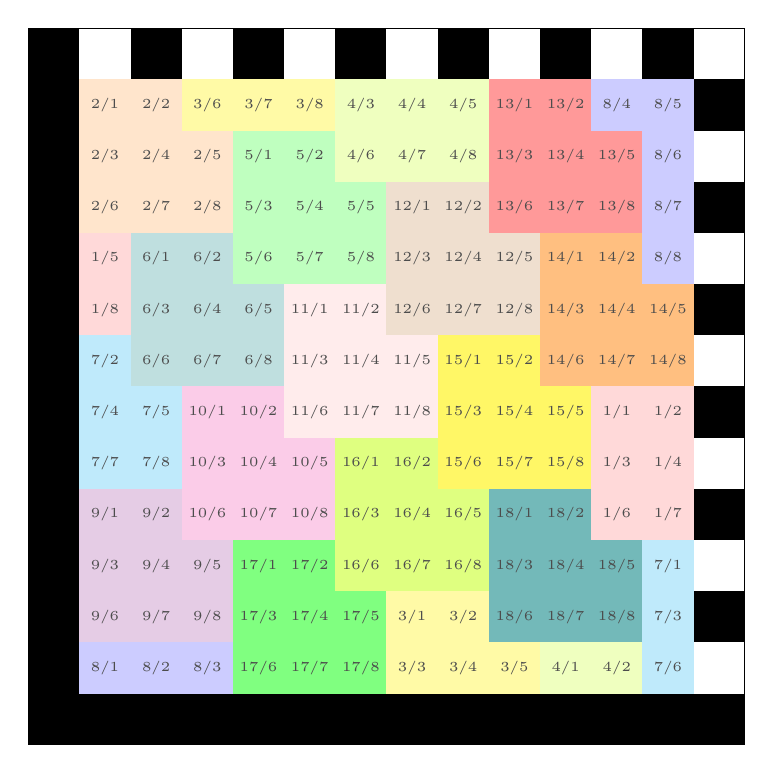
\begin{tikzpicture}[x=6.5mm, y=-6.5mm, every node/.style={font=\tiny}]
  % Symbol-Aussenrahmen 14×14
  \draw[black] (0, 0) rectangle (14, 14);
  % L-Pattern
  \foreach \c in {0,...,13}{ \fill[black] (\c, 13) rectangle (\c+1, 14); }
  \foreach \r in {0,...,12}{ \fill[black] (0, \r) rectangle (1, \r+1); }
  % Zeitsignal
  \foreach \c in {0, 2, 4, 6, 8, 10, 12}{
    \fill[black] (\c, 0) rectangle (\c+1, 1);
  }
  \foreach \r in {1, 3, 5, 7, 9, 11}{
    \fill[black] (13, \r) rectangle (14, \r+1);
  }
  % Hilfsraster für Datenbereich
  \foreach \i in {1,...,13}{
    \draw[gray!40, very thin] (\i, 1) -- (\i, 13);
    \draw[gray!40, very thin] (1, \i) -- (13, \i);
  }
  % Inhalt aus Generator
  % Auto-generiert von gen_anhang.py — n_inner=12, n_codewords=18
  \fill[orange!20] (1,1) rectangle (2,2);
  \node[font=\tiny, black!70] at (1.5,1.5) {2/1};
  \fill[orange!20] (2,1) rectangle (3,2);
  \node[font=\tiny, black!70] at (2.5,1.5) {2/2};
  \fill[yellow!35] (3,1) rectangle (4,2);
  \node[font=\tiny, black!70] at (3.5,1.5) {3/6};
  \fill[yellow!35] (4,1) rectangle (5,2);
  \node[font=\tiny, black!70] at (4.5,1.5) {3/7};
  \fill[yellow!35] (5,1) rectangle (6,2);
  \node[font=\tiny, black!70] at (5.5,1.5) {3/8};
  \fill[lime!25] (6,1) rectangle (7,2);
  \node[font=\tiny, black!70] at (6.5,1.5) {4/3};
  \fill[lime!25] (7,1) rectangle (8,2);
  \node[font=\tiny, black!70] at (7.5,1.5) {4/4};
  \fill[lime!25] (8,1) rectangle (9,2);
  \node[font=\tiny, black!70] at (8.5,1.5) {4/5};
  \fill[red!40] (9,1) rectangle (10,2);
  \node[font=\tiny, black!70] at (9.5,1.5) {13/1};
  \fill[red!40] (10,1) rectangle (11,2);
  \node[font=\tiny, black!70] at (10.5,1.5) {13/2};
  \fill[blue!20] (11,1) rectangle (12,2);
  \node[font=\tiny, black!70] at (11.5,1.5) {8/4};
  \fill[blue!20] (12,1) rectangle (13,2);
  \node[font=\tiny, black!70] at (12.5,1.5) {8/5};
  \fill[orange!20] (1,2) rectangle (2,3);
  \node[font=\tiny, black!70] at (1.5,2.5) {2/3};
  \fill[orange!20] (2,2) rectangle (3,3);
  \node[font=\tiny, black!70] at (2.5,2.5) {2/4};
  \fill[orange!20] (3,2) rectangle (4,3);
  \node[font=\tiny, black!70] at (3.5,2.5) {2/5};
  \fill[green!25] (4,2) rectangle (5,3);
  \node[font=\tiny, black!70] at (4.5,2.5) {5/1};
  \fill[green!25] (5,2) rectangle (6,3);
  \node[font=\tiny, black!70] at (5.5,2.5) {5/2};
  \fill[lime!25] (6,2) rectangle (7,3);
  \node[font=\tiny, black!70] at (6.5,2.5) {4/6};
  \fill[lime!25] (7,2) rectangle (8,3);
  \node[font=\tiny, black!70] at (7.5,2.5) {4/7};
  \fill[lime!25] (8,2) rectangle (9,3);
  \node[font=\tiny, black!70] at (8.5,2.5) {4/8};
  \fill[red!40] (9,2) rectangle (10,3);
  \node[font=\tiny, black!70] at (9.5,2.5) {13/3};
  \fill[red!40] (10,2) rectangle (11,3);
  \node[font=\tiny, black!70] at (10.5,2.5) {13/4};
  \fill[red!40] (11,2) rectangle (12,3);
  \node[font=\tiny, black!70] at (11.5,2.5) {13/5};
  \fill[blue!20] (12,2) rectangle (13,3);
  \node[font=\tiny, black!70] at (12.5,2.5) {8/6};
  \fill[orange!20] (1,3) rectangle (2,4);
  \node[font=\tiny, black!70] at (1.5,3.5) {2/6};
  \fill[orange!20] (2,3) rectangle (3,4);
  \node[font=\tiny, black!70] at (2.5,3.5) {2/7};
  \fill[orange!20] (3,3) rectangle (4,4);
  \node[font=\tiny, black!70] at (3.5,3.5) {2/8};
  \fill[green!25] (4,3) rectangle (5,4);
  \node[font=\tiny, black!70] at (4.5,3.5) {5/3};
  \fill[green!25] (5,3) rectangle (6,4);
  \node[font=\tiny, black!70] at (5.5,3.5) {5/4};
  \fill[green!25] (6,3) rectangle (7,4);
  \node[font=\tiny, black!70] at (6.5,3.5) {5/5};
  \fill[brown!25] (7,3) rectangle (8,4);
  \node[font=\tiny, black!70] at (7.5,3.5) {12/1};
  \fill[brown!25] (8,3) rectangle (9,4);
  \node[font=\tiny, black!70] at (8.5,3.5) {12/2};
  \fill[red!40] (9,3) rectangle (10,4);
  \node[font=\tiny, black!70] at (9.5,3.5) {13/6};
  \fill[red!40] (10,3) rectangle (11,4);
  \node[font=\tiny, black!70] at (10.5,3.5) {13/7};
  \fill[red!40] (11,3) rectangle (12,4);
  \node[font=\tiny, black!70] at (11.5,3.5) {13/8};
  \fill[blue!20] (12,3) rectangle (13,4);
  \node[font=\tiny, black!70] at (12.5,3.5) {8/7};
  \fill[red!15] (1,4) rectangle (2,5);
  \node[font=\tiny, black!70] at (1.5,4.5) {1/5};
  \fill[teal!25] (2,4) rectangle (3,5);
  \node[font=\tiny, black!70] at (2.5,4.5) {6/1};
  \fill[teal!25] (3,4) rectangle (4,5);
  \node[font=\tiny, black!70] at (3.5,4.5) {6/2};
  \fill[green!25] (4,4) rectangle (5,5);
  \node[font=\tiny, black!70] at (4.5,4.5) {5/6};
  \fill[green!25] (5,4) rectangle (6,5);
  \node[font=\tiny, black!70] at (5.5,4.5) {5/7};
  \fill[green!25] (6,4) rectangle (7,5);
  \node[font=\tiny, black!70] at (6.5,4.5) {5/8};
  \fill[brown!25] (7,4) rectangle (8,5);
  \node[font=\tiny, black!70] at (7.5,4.5) {12/3};
  \fill[brown!25] (8,4) rectangle (9,5);
  \node[font=\tiny, black!70] at (8.5,4.5) {12/4};
  \fill[brown!25] (9,4) rectangle (10,5);
  \node[font=\tiny, black!70] at (9.5,4.5) {12/5};
  \fill[orange!50] (10,4) rectangle (11,5);
  \node[font=\tiny, black!70] at (10.5,4.5) {14/1};
  \fill[orange!50] (11,4) rectangle (12,5);
  \node[font=\tiny, black!70] at (11.5,4.5) {14/2};
  \fill[blue!20] (12,4) rectangle (13,5);
  \node[font=\tiny, black!70] at (12.5,4.5) {8/8};
  \fill[red!15] (1,5) rectangle (2,6);
  \node[font=\tiny, black!70] at (1.5,5.5) {1/8};
  \fill[teal!25] (2,5) rectangle (3,6);
  \node[font=\tiny, black!70] at (2.5,5.5) {6/3};
  \fill[teal!25] (3,5) rectangle (4,6);
  \node[font=\tiny, black!70] at (3.5,5.5) {6/4};
  \fill[teal!25] (4,5) rectangle (5,6);
  \node[font=\tiny, black!70] at (4.5,5.5) {6/5};
  \fill[pink!30] (5,5) rectangle (6,6);
  \node[font=\tiny, black!70] at (5.5,5.5) {11/1};
  \fill[pink!30] (6,5) rectangle (7,6);
  \node[font=\tiny, black!70] at (6.5,5.5) {11/2};
  \fill[brown!25] (7,5) rectangle (8,6);
  \node[font=\tiny, black!70] at (7.5,5.5) {12/6};
  \fill[brown!25] (8,5) rectangle (9,6);
  \node[font=\tiny, black!70] at (8.5,5.5) {12/7};
  \fill[brown!25] (9,5) rectangle (10,6);
  \node[font=\tiny, black!70] at (9.5,5.5) {12/8};
  \fill[orange!50] (10,5) rectangle (11,6);
  \node[font=\tiny, black!70] at (10.5,5.5) {14/3};
  \fill[orange!50] (11,5) rectangle (12,6);
  \node[font=\tiny, black!70] at (11.5,5.5) {14/4};
  \fill[orange!50] (12,5) rectangle (13,6);
  \node[font=\tiny, black!70] at (12.5,5.5) {14/5};
  \fill[cyan!25] (1,6) rectangle (2,7);
  \node[font=\tiny, black!70] at (1.5,6.5) {7/2};
  \fill[teal!25] (2,6) rectangle (3,7);
  \node[font=\tiny, black!70] at (2.5,6.5) {6/6};
  \fill[teal!25] (3,6) rectangle (4,7);
  \node[font=\tiny, black!70] at (3.5,6.5) {6/7};
  \fill[teal!25] (4,6) rectangle (5,7);
  \node[font=\tiny, black!70] at (4.5,6.5) {6/8};
  \fill[pink!30] (5,6) rectangle (6,7);
  \node[font=\tiny, black!70] at (5.5,6.5) {11/3};
  \fill[pink!30] (6,6) rectangle (7,7);
  \node[font=\tiny, black!70] at (6.5,6.5) {11/4};
  \fill[pink!30] (7,6) rectangle (8,7);
  \node[font=\tiny, black!70] at (7.5,6.5) {11/5};
  \fill[yellow!60] (8,6) rectangle (9,7);
  \node[font=\tiny, black!70] at (8.5,6.5) {15/1};
  \fill[yellow!60] (9,6) rectangle (10,7);
  \node[font=\tiny, black!70] at (9.5,6.5) {15/2};
  \fill[orange!50] (10,6) rectangle (11,7);
  \node[font=\tiny, black!70] at (10.5,6.5) {14/6};
  \fill[orange!50] (11,6) rectangle (12,7);
  \node[font=\tiny, black!70] at (11.5,6.5) {14/7};
  \fill[orange!50] (12,6) rectangle (13,7);
  \node[font=\tiny, black!70] at (12.5,6.5) {14/8};
  \fill[cyan!25] (1,7) rectangle (2,8);
  \node[font=\tiny, black!70] at (1.5,7.5) {7/4};
  \fill[cyan!25] (2,7) rectangle (3,8);
  \node[font=\tiny, black!70] at (2.5,7.5) {7/5};
  \fill[magenta!20] (3,7) rectangle (4,8);
  \node[font=\tiny, black!70] at (3.5,7.5) {10/1};
  \fill[magenta!20] (4,7) rectangle (5,8);
  \node[font=\tiny, black!70] at (4.5,7.5) {10/2};
  \fill[pink!30] (5,7) rectangle (6,8);
  \node[font=\tiny, black!70] at (5.5,7.5) {11/6};
  \fill[pink!30] (6,7) rectangle (7,8);
  \node[font=\tiny, black!70] at (6.5,7.5) {11/7};
  \fill[pink!30] (7,7) rectangle (8,8);
  \node[font=\tiny, black!70] at (7.5,7.5) {11/8};
  \fill[yellow!60] (8,7) rectangle (9,8);
  \node[font=\tiny, black!70] at (8.5,7.5) {15/3};
  \fill[yellow!60] (9,7) rectangle (10,8);
  \node[font=\tiny, black!70] at (9.5,7.5) {15/4};
  \fill[yellow!60] (10,7) rectangle (11,8);
  \node[font=\tiny, black!70] at (10.5,7.5) {15/5};
  \fill[red!15] (11,7) rectangle (12,8);
  \node[font=\tiny, black!70] at (11.5,7.5) {1/1};
  \fill[red!15] (12,7) rectangle (13,8);
  \node[font=\tiny, black!70] at (12.5,7.5) {1/2};
  \fill[cyan!25] (1,8) rectangle (2,9);
  \node[font=\tiny, black!70] at (1.5,8.5) {7/7};
  \fill[cyan!25] (2,8) rectangle (3,9);
  \node[font=\tiny, black!70] at (2.5,8.5) {7/8};
  \fill[magenta!20] (3,8) rectangle (4,9);
  \node[font=\tiny, black!70] at (3.5,8.5) {10/3};
  \fill[magenta!20] (4,8) rectangle (5,9);
  \node[font=\tiny, black!70] at (4.5,8.5) {10/4};
  \fill[magenta!20] (5,8) rectangle (6,9);
  \node[font=\tiny, black!70] at (5.5,8.5) {10/5};
  \fill[lime!50] (6,8) rectangle (7,9);
  \node[font=\tiny, black!70] at (6.5,8.5) {16/1};
  \fill[lime!50] (7,8) rectangle (8,9);
  \node[font=\tiny, black!70] at (7.5,8.5) {16/2};
  \fill[yellow!60] (8,8) rectangle (9,9);
  \node[font=\tiny, black!70] at (8.5,8.5) {15/6};
  \fill[yellow!60] (9,8) rectangle (10,9);
  \node[font=\tiny, black!70] at (9.5,8.5) {15/7};
  \fill[yellow!60] (10,8) rectangle (11,9);
  \node[font=\tiny, black!70] at (10.5,8.5) {15/8};
  \fill[red!15] (11,8) rectangle (12,9);
  \node[font=\tiny, black!70] at (11.5,8.5) {1/3};
  \fill[red!15] (12,8) rectangle (13,9);
  \node[font=\tiny, black!70] at (12.5,8.5) {1/4};
  \fill[violet!20] (1,9) rectangle (2,10);
  \node[font=\tiny, black!70] at (1.5,9.5) {9/1};
  \fill[violet!20] (2,9) rectangle (3,10);
  \node[font=\tiny, black!70] at (2.5,9.5) {9/2};
  \fill[magenta!20] (3,9) rectangle (4,10);
  \node[font=\tiny, black!70] at (3.5,9.5) {10/6};
  \fill[magenta!20] (4,9) rectangle (5,10);
  \node[font=\tiny, black!70] at (4.5,9.5) {10/7};
  \fill[magenta!20] (5,9) rectangle (6,10);
  \node[font=\tiny, black!70] at (5.5,9.5) {10/8};
  \fill[lime!50] (6,9) rectangle (7,10);
  \node[font=\tiny, black!70] at (6.5,9.5) {16/3};
  \fill[lime!50] (7,9) rectangle (8,10);
  \node[font=\tiny, black!70] at (7.5,9.5) {16/4};
  \fill[lime!50] (8,9) rectangle (9,10);
  \node[font=\tiny, black!70] at (8.5,9.5) {16/5};
  \fill[teal!55] (9,9) rectangle (10,10);
  \node[font=\tiny, black!70] at (9.5,9.5) {18/1};
  \fill[teal!55] (10,9) rectangle (11,10);
  \node[font=\tiny, black!70] at (10.5,9.5) {18/2};
  \fill[red!15] (11,9) rectangle (12,10);
  \node[font=\tiny, black!70] at (11.5,9.5) {1/6};
  \fill[red!15] (12,9) rectangle (13,10);
  \node[font=\tiny, black!70] at (12.5,9.5) {1/7};
  \fill[violet!20] (1,10) rectangle (2,11);
  \node[font=\tiny, black!70] at (1.5,10.5) {9/3};
  \fill[violet!20] (2,10) rectangle (3,11);
  \node[font=\tiny, black!70] at (2.5,10.5) {9/4};
  \fill[violet!20] (3,10) rectangle (4,11);
  \node[font=\tiny, black!70] at (3.5,10.5) {9/5};
  \fill[green!50] (4,10) rectangle (5,11);
  \node[font=\tiny, black!70] at (4.5,10.5) {17/1};
  \fill[green!50] (5,10) rectangle (6,11);
  \node[font=\tiny, black!70] at (5.5,10.5) {17/2};
  \fill[lime!50] (6,10) rectangle (7,11);
  \node[font=\tiny, black!70] at (6.5,10.5) {16/6};
  \fill[lime!50] (7,10) rectangle (8,11);
  \node[font=\tiny, black!70] at (7.5,10.5) {16/7};
  \fill[lime!50] (8,10) rectangle (9,11);
  \node[font=\tiny, black!70] at (8.5,10.5) {16/8};
  \fill[teal!55] (9,10) rectangle (10,11);
  \node[font=\tiny, black!70] at (9.5,10.5) {18/3};
  \fill[teal!55] (10,10) rectangle (11,11);
  \node[font=\tiny, black!70] at (10.5,10.5) {18/4};
  \fill[teal!55] (11,10) rectangle (12,11);
  \node[font=\tiny, black!70] at (11.5,10.5) {18/5};
  \fill[cyan!25] (12,10) rectangle (13,11);
  \node[font=\tiny, black!70] at (12.5,10.5) {7/1};
  \fill[violet!20] (1,11) rectangle (2,12);
  \node[font=\tiny, black!70] at (1.5,11.5) {9/6};
  \fill[violet!20] (2,11) rectangle (3,12);
  \node[font=\tiny, black!70] at (2.5,11.5) {9/7};
  \fill[violet!20] (3,11) rectangle (4,12);
  \node[font=\tiny, black!70] at (3.5,11.5) {9/8};
  \fill[green!50] (4,11) rectangle (5,12);
  \node[font=\tiny, black!70] at (4.5,11.5) {17/3};
  \fill[green!50] (5,11) rectangle (6,12);
  \node[font=\tiny, black!70] at (5.5,11.5) {17/4};
  \fill[green!50] (6,11) rectangle (7,12);
  \node[font=\tiny, black!70] at (6.5,11.5) {17/5};
  \fill[yellow!35] (7,11) rectangle (8,12);
  \node[font=\tiny, black!70] at (7.5,11.5) {3/1};
  \fill[yellow!35] (8,11) rectangle (9,12);
  \node[font=\tiny, black!70] at (8.5,11.5) {3/2};
  \fill[teal!55] (9,11) rectangle (10,12);
  \node[font=\tiny, black!70] at (9.5,11.5) {18/6};
  \fill[teal!55] (10,11) rectangle (11,12);
  \node[font=\tiny, black!70] at (10.5,11.5) {18/7};
  \fill[teal!55] (11,11) rectangle (12,12);
  \node[font=\tiny, black!70] at (11.5,11.5) {18/8};
  \fill[cyan!25] (12,11) rectangle (13,12);
  \node[font=\tiny, black!70] at (12.5,11.5) {7/3};
  \fill[blue!20] (1,12) rectangle (2,13);
  \node[font=\tiny, black!70] at (1.5,12.5) {8/1};
  \fill[blue!20] (2,12) rectangle (3,13);
  \node[font=\tiny, black!70] at (2.5,12.5) {8/2};
  \fill[blue!20] (3,12) rectangle (4,13);
  \node[font=\tiny, black!70] at (3.5,12.5) {8/3};
  \fill[green!50] (4,12) rectangle (5,13);
  \node[font=\tiny, black!70] at (4.5,12.5) {17/6};
  \fill[green!50] (5,12) rectangle (6,13);
  \node[font=\tiny, black!70] at (5.5,12.5) {17/7};
  \fill[green!50] (6,12) rectangle (7,13);
  \node[font=\tiny, black!70] at (6.5,12.5) {17/8};
  \fill[yellow!35] (7,12) rectangle (8,13);
  \node[font=\tiny, black!70] at (7.5,12.5) {3/3};
  \fill[yellow!35] (8,12) rectangle (9,13);
  \node[font=\tiny, black!70] at (8.5,12.5) {3/4};
  \fill[yellow!35] (9,12) rectangle (10,13);
  \node[font=\tiny, black!70] at (9.5,12.5) {3/5};
  \fill[lime!25] (10,12) rectangle (11,13);
  \node[font=\tiny, black!70] at (10.5,12.5) {4/1};
  \fill[lime!25] (11,12) rectangle (12,13);
  \node[font=\tiny, black!70] at (11.5,12.5) {4/2};
  \fill[cyan!25] (12,12) rectangle (13,13);
  \node[font=\tiny, black!70] at (12.5,12.5) {7/6};

\end{tikzpicture}
\end{center}

\paragraph{Lesehilfe} CW~1 = $230$ (Latch nach C40), CW~2--7 = drei
C40-Triplet-Paare, CW~8 = $254$ (Unlatch zurück), CW~9--18 = 10~ECC.
Bei dieser Größe sind die Pastellfarben recht eng beieinander —
zwei Buntstift-Sets nebeneinander legen hilft.
